\hypertarget{dataframes-and-series}{%
\chapter{DataFrames and Series}\label{dataframes-and-series}}

This chapter introduces Pandas, a Python library that provides functions
for reading and writing data files, exploring and analyzing data, and
generating visualizations. And it provides two new types for working
with data, \passthrough{\lstinline!DataFrame!} and
\passthrough{\lstinline!Series!}.

We will use these tools to answer a data question: what is the average
birth weight of babies in the United States? This example will
demonstrate important steps in almost any data science project:

\begin{enumerate}
\def\labelenumi{\arabic{enumi}.}
\item
  Identifying data that can answer a question.
\item
  Obtaining the data and loading it in Python.
\item
  Checking the data and dealing with errors.
\item
  Selecting relevant subsets from the data.
\item
  Using histograms to visualize a distribution of values.
\item
  Using summary statistics to describe the data in a way that best
  answers the question.
\item
  Considering possible sources of error and limitations in our
  conclusions.
\end{enumerate}

Let's start by getting the data.

\hypertarget{reading-the-data}{%
\section{Reading the Data}\label{reading-the-data}}

We'll use data from the National Survey of Family Growth (NSFG), which
is available from the National Center for Health Statistics at
\url{https://www.cdc.gov/nchs/nsfg/index.htm}.

To download the data, you have to agree to the Data User's Agreement at
\url{https://www.cdc.gov/nchs/data_access/ftp_dua.htm}. You should read
those terms carefully, but let me draw your attention to what I think is
the most important one:

\begin{quote}
Make no attempt to learn the identity of any person or establishment
included in these data.
\end{quote}

NSFG respondents provide honest answers to questions of the most
personal nature with the expectation that their identities will not be
revealed. As ethical data scientists, we should respect their privacy
and adhere to the terms of use.

Respondents to the NSFG provide general information about themselves,
which is stored in the respondent file, and information about each time
they have been pregnant, which is stored in the pregnancy file.

We will work with the pregnancy file, which contains one row for each
pregnancy and one column for each of the 248 variables. Each variable
represents responses to a question on the NSFG questionnaire.

The data is stored in a fixed-width format, which means that every row
is the same length and each variable spans a fixed range of characters
(see
\url{https://www.ibm.com/docs/en/baw/19.x?topic=formats-fixed-width-format}).
For example, the first six characters in each row represent a variable
called \passthrough{\lstinline!CASEID!}, which is a unique identifier
for each respondent; the next two characters represent
\passthrough{\lstinline!PREGORDR!}, which indicates whether a pregnancy
is the respondent's first, second, etc.

To read this data, we need a \textbf{data dictionary}, which specifies
the names of the variables and the range of characters where each
variable appears. The data and the data dictionary are available in
separate files.

\begin{lstlisting}[]
dict_file = '2015_2017_FemPregSetup.dct'
data_file = '2015_2017_FemPregData.dat'
\end{lstlisting}

Pandas can read data in most common formats, including CSV, Excel, and
fixed-width format, but it cannot read the data dictionary, which is in
Stata format. For that, we'll use a Python library called
\passthrough{\lstinline!statadict!}.

From \passthrough{\lstinline!statadict!}, we'll import
\passthrough{\lstinline!parse\_stata\_dict!}, which reads the data
dictionary.

\begin{lstlisting}[]
from statadict import parse_stata_dict

stata_dict = parse_stata_dict(dict_file)
stata_dict
(@\dashfill@)
@@@<statadict.base.StataDict at 0x7fc25535b490>@@@
\end{lstlisting}

The result is an object that contains

\begin{itemize}
\item
  \passthrough{\lstinline!names!}, which is a list of variable names,
  and
\item
  \passthrough{\lstinline!colspecs!}, which is a list of tuples.
\end{itemize}

Each tuple in \passthrough{\lstinline!colspecs!} specifies the first and
last column where a variable appears.

These values are exactly the arguments we need to use
\passthrough{\lstinline!read\_fwf!}, which is the Pandas function that
reads a file in fixed-width format.

\begin{lstlisting}[]
import pandas as pd

nsfg = pd.read_fwf(data_file, 
                   names=stata_dict.names, 
                   colspecs=stata_dict.colspecs)
type(nsfg)
(@\dashfill@)
@@@pandas.core.frame.DataFrame@@@
\end{lstlisting}

The result from \passthrough{\lstinline!read\_fwf()!} is a
\passthrough{\lstinline!DataFrame!}, which is the primary type Pandas
uses to store data. \passthrough{\lstinline!DataFrame!} has a method
called \passthrough{\lstinline!head()!} that shows the first 5 rows:

\begin{lstlisting}[]
nsfg.head()
\end{lstlisting}

\begin{tabular}{lrrrrrrr}
\midrule
{} &  CASEID &  PREGORDR &  HOWPREG\_N &  HOWPREG\_P &  MOSCURRP \\
\midrule
0 &   70627 &         1 &        NaN &        NaN &       NaN  \\
1 &   70627 &         2 &        NaN &        NaN &       NaN  \\
2 &   70627 &         3 &        NaN &        NaN &       NaN  \\
3 &   70628 &         1 &        NaN &        NaN &       NaN  \\
4 &   70628 &         2 &        NaN &        NaN &       NaN  \\
\midrule
\end{tabular}

Only the first five columns are shown here.
The first two columns are is \passthrough{\lstinline!CASEID!} and
\passthrough{\lstinline!PREGORDR!}, which I mentioned earlier. The first
three rows have the same \passthrough{\lstinline!CASEID!}, so this
respondent reported three pregnancies; the values of
\passthrough{\lstinline!PREGORDR!} indicate that they are the first,
second, and third pregnancies, in that order.
We will learn more about the other variables as we go along.

In addition to methods like \passthrough{\lstinline!head!}, a
\passthrough{\lstinline!Dataframe!} object has several
\textbf{attributes}, which are variables associated with the object. For
example, \passthrough{\lstinline!nsfg!} has an attribute called
\passthrough{\lstinline!shape!}, which is a tuple containing the number
of rows and columns:

\begin{lstlisting}[]
nsfg.shape
(@\dashfill@)
@@@(9553, 248)@@@
\end{lstlisting}

There are 9553 rows in this dataset, one for each pregnancy, and 248
columns, one for each variable.

\passthrough{\lstinline!nsfg!} also has an attribute called
\passthrough{\lstinline!columns!}, which contains the column names:

\begin{lstlisting}[]
nsfg.columns
(@\dashfill@)
@@@Index(['CASEID', 'PREGORDR', 'HOWPREG_N', 'HOWPREG_P', 'MOSCURRP', 'NOWPRGDK',
       'PREGEND1', 'PREGEND2', 'HOWENDDK', 'NBRNALIV',
       ...
       'SECU', 'SEST', 'CMINTVW', 'CMLSTYR', 'CMJAN3YR', 'CMJAN4YR',
       'CMJAN5YR', 'QUARTER', 'PHASE', 'INTVWYEAR'],
      dtype='object', length=248)@@@
\end{lstlisting}

The column names are stored in an \passthrough{\lstinline!Index!}, which
is another Pandas type, similar to a list.

Based on the column names, you might be able to guess what some of the
variables are, but in general you have to read the documentation.

When you work with datasets like the NSFG, it is important to read the
documentation carefully. If you interpret a variable incorrectly, you
can generate nonsense results and never realize it. So, before we start
looking at data, let's get familiar with the NSFG codebook, which
describes every variable. You can download the codebook for this dataset
from
\url{https://github.com/AllenDowney/ElementsOfDataScience/raw/master/data/2015-2017_NSFG_FemPregFile_Codebook-508.pdf}.

If you search that document for ``weigh at birth'' you should find these
variables related to birth weight.

\begin{itemize}
\item
  \passthrough{\lstinline!BIRTHWGT\_LB1!}: Birthweight in Pounds - 1st
  baby from this pregnancy
\item
  \passthrough{\lstinline!BIRTHWGT\_OZ1!}: Birthweight in Ounces - 1st
  baby from this pregnancy
\end{itemize}

There are similar variables for a 2nd or 3rd baby, in the case of twins
or triplets. For now we will focus on the first baby from each
pregnancy, and we will come back to the issue of multiple births.

\hypertarget{series}{%
\section{Series}\label{series}}

In many ways a \passthrough{\lstinline!DataFrame!} is like a Python
dictionary, where the column names are the keys and the columns are the
values. You can select a column from a
\passthrough{\lstinline!DataFrame!} using the bracket operator, with a
string as the key.

\begin{lstlisting}[]
pounds = nsfg['BIRTHWGT_LB1']
type(pounds)
(@\dashfill@)
@@@pandas.core.series.Series@@@
\end{lstlisting}

The result is a \passthrough{\lstinline!Series!}, which is a Pandas type
that represents a single column of data. In this case the
\passthrough{\lstinline!Series!} contains the birth weight, in pounds,
for each live birth.

\passthrough{\lstinline!head!} shows the first five values in the
\passthrough{\lstinline!Series!}, the name of the
\passthrough{\lstinline!Series!}, and the data type:

\begin{lstlisting}[]
pounds.head()
\end{lstlisting}

\begin{tabular}{lr}
\midrule
{} &  BIRTHWGT\_LB1 \\
\midrule
0 &           7.0 \\
1 &           NaN \\
2 &           9.0 \\
3 &           6.0 \\
4 &           7.0 \\
\midrule
\end{tabular}

One of the values is \passthrough{\lstinline!NaN!}, which stands for
``Not a Number''. \passthrough{\lstinline!NaN!} is a special value used
to indicate invalid or missing data. In this example, the pregnancy did
not end in live birth, so birth weight is inapplicable.

\textbf{Exercise:} The variable \passthrough{\lstinline!BIRTHWGT\_OZ1!}
contains the ounces part of birth weight.

Select the column \passthrough{\lstinline!'BIRTHWGT\_OZ1'!} from the
\passthrough{\lstinline!nsfg!} \passthrough{\lstinline!DataFrame!} and
assign it to a new variable called \passthrough{\lstinline!ounces!}.
Then display the first 5 elements of \passthrough{\lstinline!ounces!}.

\textbf{Exercise:} The Pandas types we have seen so far are
\passthrough{\lstinline!DataFrame!}, \passthrough{\lstinline!Index!},
and \passthrough{\lstinline!Series!}. You can find the documentation of
these types at:

\begin{itemize}
\item
  \passthrough{\lstinline!DataFrame!}:
  \url{https://pandas.pydata.org/pandas-docs/stable/reference/api/pandas.DataFrame.html}
\item
  \passthrough{\lstinline!Index!}:
  \url{https://pandas.pydata.org/pandas-docs/stable/reference/api/pandas.Index.html}
\item
  \passthrough{\lstinline!Series!}:
  \url{https://pandas.pydata.org/pandas-docs/stable/reference/api/pandas.Series.html}
\end{itemize}

This documentation can be overwhelming; I don't recommend trying to read
it all now. But you might want to skim it so you know where to look
later.

\hypertarget{validation}{%
\section{Validation}\label{validation}}

At this point we have identified the columns we need to answer the
question and assigned them to variables named
\passthrough{\lstinline!pounds!} and \passthrough{\lstinline!ounces!}.

\begin{lstlisting}[]
pounds = nsfg['BIRTHWGT_LB1']
ounces = nsfg['BIRTHWGT_OZ1']
\end{lstlisting}

Before we do anything with this data, we have to validate it. One part
of validation is confirming that we are interpreting the data correctly.

We can use the \passthrough{\lstinline!value\_counts!} method to see
what values appear in \passthrough{\lstinline!pounds!} and how many
times each value appears.

\begin{lstlisting}[]
pounds.value_counts()
\end{lstlisting}

\begin{tabular}{lr}
\midrule
{} &  BIRTHWGT\_LB1 \\
\midrule
7.0  &          2268 \\
6.0  &          1644 \\
8.0  &          1287 \\
5.0  &           570 \\
9.0  &           396 \\
4.0  &           179 \\
99.0 &            89 \\
10.0 &            82 \\
3.0  &            76 \\
2.0  &            46 \\
1.0  &            28 \\
11.0 &            17 \\
0.0  &             2 \\
12.0 &             2 \\
98.0 &             2 \\
13.0 &             1 \\
14.0 &             1 \\
\midrule
\end{tabular}

By default, the results are sorted with the most frequent value first,
but we can use \passthrough{\lstinline!sort\_index!} to sort them by
value instead, with the lightest babies first and heaviest babies last.

\begin{lstlisting}[]
pounds.value_counts().sort_index()
\end{lstlisting}

\begin{tabular}{lr}
\midrule
{} &  BIRTHWGT\_LB1 \\
\midrule
0.0  &             2 \\
1.0  &            28 \\
2.0  &            46 \\
3.0  &            76 \\
4.0  &           179 \\
5.0  &           570 \\
6.0  &          1644 \\
7.0  &          2268 \\
8.0  &          1287 \\
9.0  &           396 \\
10.0 &            82 \\
11.0 &            17 \\
12.0 &             2 \\
13.0 &             1 \\
14.0 &             1 \\
98.0 &             2 \\
99.0 &            89 \\
\midrule
\end{tabular}

As we'd expect, the most frequent values are 6-8 pounds, but there are
some very light babies, a few very heavy babies, and two special values,
98, and 99. According to the codebook, these values indicate that the
respondent declined to answer the question (98) or did not know (99).

We can validate the results by comparing them to the codebook, which
lists the values and their frequencies.

\begin{longtable}[]{@{}lll@{}}
\midrule()
value & label & Total \\
\midrule()
\endhead
. & INAPPLICABLE & 2863 \\
0-5 & UNDER 6 POUNDS & 901 \\
6 & 6 POUNDS & 1644 \\
7 & 7 POUNDS & 2268 \\
8 & 8 POUNDS & 1287 \\
9-95 & 9 POUNDS OR MORE & 499 \\
98 & Refused & 2 \\
99 & Don't know & 89 \\
& Total & 9553 \\
\midrule()
\end{longtable}

The results from \passthrough{\lstinline!value\_counts!} agree with the
codebook, so we have some confidence that we are reading and
interpreting the data correctly.

\textbf{Exercise:} In the \passthrough{\lstinline!nsfg!}
\passthrough{\lstinline!DataFrame!}, the column
\passthrough{\lstinline!'OUTCOME'!} encodes the outcome of each
pregnancy as shown below:

\begin{longtable}[]{@{}ll@{}}
\midrule()
Value & Meaning \\
\midrule()
\endhead
1 & Live birth \\
2 & Induced abortion \\
3 & Stillbirth \\
4 & Miscarriage \\
5 & Ectopic pregnancy \\
6 & Current pregnancy \\
\midrule()
\end{longtable}

Use \passthrough{\lstinline!value\_counts!} to display the values in
this column and how many times each value appears. Are the results
consistent with the codebook?

\hypertarget{summary-statistics}{%
\section{Summary Statistics}\label{summary-statistics}}

Another way to validate the data is with
\passthrough{\lstinline!describe!}, which computes statistics that
summarize the data, like the mean, standard deviation, minimum, and
maximum.

Here are the results for \passthrough{\lstinline!pounds!}.

\begin{lstlisting}[]
pounds.describe()
\end{lstlisting}

\begin{tabular}{lr}
\midrule
{} &  BIRTHWGT\_LB1 \\
\midrule
count &   6690.000000 \\
mean  &      8.008819 \\
std   &     10.771360 \\
min   &      0.000000 \\
25\%   &      6.000000 \\
50\%   &      7.000000 \\
75\%   &      8.000000 \\
max   &     99.000000 \\
\midrule
\end{tabular}

\passthrough{\lstinline!count!} is the number of values, not including
\passthrough{\lstinline!NaN!}. For this variable, there are 6690 value
that are not \passthrough{\lstinline!NaN!}.

\passthrough{\lstinline!mean!} and \passthrough{\lstinline!std!} are the
mean and standard deviation. \passthrough{\lstinline!min!} and
\passthrough{\lstinline!max!} are the minimum and maximum values, and in
between are the 25th, 50th, and 75th percentiles. The 50th percentile is
the median.

The mean is about \passthrough{\lstinline!8.05!}, but that doesn't mean
much because it includes the special values 98 and 99. Before we can
really compute the mean, we have to replace those values with
\passthrough{\lstinline!NaN!} to identify them as missing data.

The \passthrough{\lstinline!replace()!} method does what we want:

\begin{lstlisting}[]
import numpy as np

pounds_clean = pounds.replace([98, 99], np.nan)
\end{lstlisting}

\passthrough{\lstinline!replace!} takes a list of the values we want to
replace and the value we want to replace them with.
\passthrough{\lstinline!np.nan!} means we are getting the special value
\passthrough{\lstinline!NaN!} from the NumPy library, which is imported
as \passthrough{\lstinline!np!}.

The result from \passthrough{\lstinline!replace()!} is a new
\passthrough{\lstinline!Series!}, which I assign to
\passthrough{\lstinline!pounds\_clean!}. If we run
\passthrough{\lstinline!describe!} again, we see that
\passthrough{\lstinline!count!} is smaller now because it includes only
the valid values.

\begin{lstlisting}[]
pounds_clean.describe()
\end{lstlisting}

\begin{tabular}{lr}
\midrule
{} &  BIRTHWGT\_LB1 \\
\midrule
count &   6599.000000 \\
mean  &      6.754357 \\
std   &      1.383268 \\
min   &      0.000000 \\
25\%   &      6.000000 \\
50\%   &      7.000000 \\
75\%   &      8.000000 \\
max   &     14.000000 \\
\midrule
\end{tabular}

The mean of the new \passthrough{\lstinline!Series!} is about 6.7
pounds. Remember that the mean of the original
\passthrough{\lstinline!Series!} was more than 8 pounds. It makes a big
difference when you remove a few 99-pound babies!

\textbf{Exercise:} Use \passthrough{\lstinline!describe!} to summarize
\passthrough{\lstinline!ounces!}.\\
Then use \passthrough{\lstinline!replace!} to replace the special values
98 and 99 with NaN, and assign the result to
\passthrough{\lstinline!ounces\_clean!}. Run
\passthrough{\lstinline!describe!} again. How much does this cleaning
affect the results?

\hypertarget{series-arithmetic}{%
\section{Series Arithmetic}\label{series-arithmetic}}

Now we want to combine \passthrough{\lstinline!pounds!} and
\passthrough{\lstinline!ounces!} into a single
\passthrough{\lstinline!Series!} that contains total birth weight.
Arithmetic operators work with \passthrough{\lstinline!Series!} objects;
so, for example, to convert \passthrough{\lstinline!pounds!} to ounces,
we could write

\passthrough{\lstinline!pounds * 16!}

Then we could add in \passthrough{\lstinline!ounces!} like this

\passthrough{\lstinline!pounds * 16 + ounces!}

\textbf{Exercise:} Use \passthrough{\lstinline!pounds\_clean!} and
\passthrough{\lstinline!ounces\_clean!} to compute the total birth
weight expressed in kilograms (there are roughly 2.2 pounds per
kilogram). What is the mean birth weight in kilograms?

\textbf{Exercise:} For each pregnancy in the NSFG dataset, the variable
\passthrough{\lstinline!'AGECON'!} encodes the respondent's age at
conception, and \passthrough{\lstinline!'AGEPREG'!} the respondent's age
at the end of the pregnancy.

\begin{itemize}
\item
  Read the documentation of these variables. Are there any special
  values we have to deal with?
\item
  Select \passthrough{\lstinline!'AGECON'!} and
  \passthrough{\lstinline!'AGEPREG'!} and assign them to variables named
  \passthrough{\lstinline!agecon!} and
  \passthrough{\lstinline!agepreg!}.
\item
  Compute the difference, which is an estimate of the duration of the
  pregnancy.
\item
  Use \passthrough{\lstinline!.describe()!} to compute the mean duration
  and other summary statistics.
\end{itemize}

Based on the results, it seems like this might not be a good way to
estimate the duration of pregnancy. Why not?

\hypertarget{histograms}{%
\section{Histograms}\label{histograms}}

Let's get back to the original question: what is the average birth
weight for babies in the U.S.?\\
As an answer we \emph{could} take the results from the previous section
and compute the mean:

\begin{lstlisting}[]
pounds_clean = pounds.replace([98, 99], np.nan)
ounces_clean = ounces.replace([98, 99], np.nan)

birth_weight = pounds_clean + ounces_clean / 16
birth_weight.mean()
(@\dashfill@)
@@@7.180217889908257@@@
\end{lstlisting}

But it is risky to compute a summary statistic, like the mean, before we
look at the whole distribution of values.

A \textbf{distribution} is a set of possible values and their
frequencies. One way to visualize a distribution is a
\textbf{histogram}, which shows values on the
\passthrough{\lstinline!x!} axis and their frequencies on the
\passthrough{\lstinline!y!} axis.

\passthrough{\lstinline!Series!} provides a
\passthrough{\lstinline!hist!} method that makes histograms. And we can
use Matplotlib to label the axes.

\begin{lstlisting}[]
import matplotlib.pyplot as plt

birth_weight.hist(bins=30)
plt.xlabel('Birth weight in pounds')
plt.ylabel('Number of live births')
plt.title('Distribution of U.S. birth weight');
\end{lstlisting}

\begin{center}
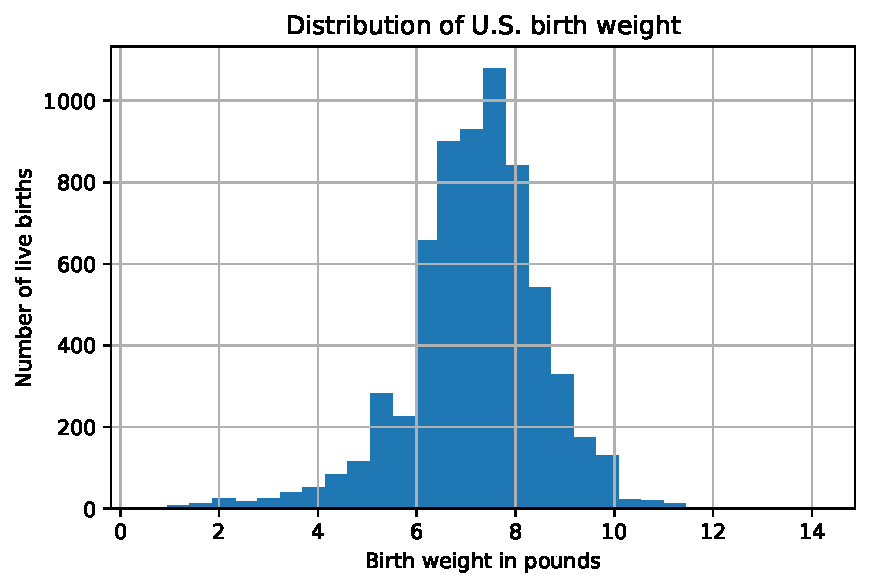
\includegraphics[width=4in]{chapters/07_dataframes_files/07_dataframes_61_0.pdf}
\end{center}

The keyword argument, \passthrough{\lstinline!bins!}, tells
\passthrough{\lstinline!hist!} to divide the range of weights into 30
intervals, called \textbf{bins}, and count how many values fall in each
bin. The \passthrough{\lstinline!x!} axis is birth weight in pounds; the
\passthrough{\lstinline!y!} axis is the number of births in each bin.

The distribution looks a little like a bell curve, but the tail is
longer on the left than on the right; that is, there are more light
babies than heavy babies. That makes sense, because the distribution
includes some babies that were born preterm.

\textbf{Exercise:} \passthrough{\lstinline!hist!} takes keyword
arguments that specify the type and appearance of the histogram. Find
the documentation of \passthrough{\lstinline!hist!} and see if you can
figure out how to plot the histogram as an unfilled line against a
background with no grid lines.

\textbf{Exercise:} As we saw in a previous exercise, the NSFG dataset
includes a column called \passthrough{\lstinline!AGECON!} that records
age at conception for each pregnancy.

\begin{itemize}
\item
  Select this column from the \passthrough{\lstinline!DataFrame!} and
  plot the histogram of the values with 20 bins.
\item
  Label the \passthrough{\lstinline!x!} and \passthrough{\lstinline!y!}
  axes appropriately.
\end{itemize}

\hypertarget{boolean-series}{%
\section{Boolean Series}\label{boolean-series}}

We have seen that the distribution of birth weights is \textbf{skewed}
to the left; that is, there are more light babies than heavy ones and
they are farther from the mean. That's because preterm babies tend to be
lighter. The most common duration for pregnancy is 39 weeks, which is
``full term''; ``preterm'' is usually defined to be less than 37 weeks.

To see which babies are preterm, we can use
\passthrough{\lstinline!PRGLNGTH!}, which records pregnancy length in
weeks and compute it to \passthrough{\lstinline!37!}.

\begin{lstlisting}[]
preterm = (nsfg['PRGLNGTH'] < 37)
preterm.dtype
(@\dashfill@)
@@@dtype('bool')@@@
\end{lstlisting}

When you compare a \passthrough{\lstinline!Series!} to a value, the
result is a Boolean \passthrough{\lstinline!Series!}; that is, a
\passthrough{\lstinline!Series!} where each element is a Boolean value,
\passthrough{\lstinline!True!} or \passthrough{\lstinline!False!}. In
this case, it's \passthrough{\lstinline!True!} for each preterm baby and
\passthrough{\lstinline!False!} otherwise. We can use
\passthrough{\lstinline!head!} to see the first 5 elements.

\begin{lstlisting}[]
preterm.head()
\end{lstlisting}

\begin{tabular}{ll}
\midrule
{} &  PRGLNGTH \\
\midrule
0 &     False \\
1 &      True \\
2 &     False \\
3 &     False \\
4 &     False \\
\midrule
\end{tabular}

If you compute the sum of a Boolean \passthrough{\lstinline!Series!}, it
treats \passthrough{\lstinline!True!} as 1 and
\passthrough{\lstinline!False!} as 0, so the sum is the number of
\passthrough{\lstinline!True!} values, which is the number of preterm
babies.

\begin{lstlisting}[]
preterm.sum()
(@\dashfill@)
@@@3675@@@
\end{lstlisting}

If you compute the mean of a Boolean \passthrough{\lstinline!Series!},
you get the \emph{fraction} of \passthrough{\lstinline!True!} values. In
this case, it's about 0.38; that is, about 38\% of the pregnancies are
less than 37 weeks.

\begin{lstlisting}[]
preterm.mean()
(@\dashfill@)
@@@0.38469590704490736@@@
\end{lstlisting}

However, this result might be misleading because it includes all
pregnancy outcomes, not just live births. We can create another Boolean
\passthrough{\lstinline!Series!} to indicate which pregnancies ended in
live birth:

\begin{lstlisting}[]
live = (nsfg['OUTCOME'] == 1)
live.mean()
(@\dashfill@)
@@@0.7006176070344394@@@
\end{lstlisting}

Now we can use the operator \passthrough{\lstinline!\&!}, which
represents the logical AND operation, to identify pregnancies where the
outcome is a live birth and preterm:

\begin{lstlisting}[]
live_preterm = (live & preterm)
live_preterm.mean()
(@\dashfill@)
@@@0.08929132209777034@@@
\end{lstlisting}

About 9\% of all pregnancies resulted in a preterm live birth.

\textbf{Exercise:} Of all live births, what fraction are preterm?

The other common logical operators are:

\begin{itemize}
\item
  \passthrough{\lstinline!|!}, which represents the logical OR
  operation; for example \passthrough{\lstinline!live | preterm!} is
  true if either \passthrough{\lstinline!live!} is true, or
  \passthrough{\lstinline!preterm!} is true, or both.
\item
  \passthrough{\lstinline!\~!}, which represents the logical NOT
  operation; for example \passthrough{\lstinline!\~live!} is true if
  \passthrough{\lstinline!live!} is false or
  \passthrough{\lstinline!NaN!}.
\end{itemize}

The logical operators treat \passthrough{\lstinline!NaN!} the same as
\passthrough{\lstinline!False!}, so you should be careful about using
the NOT operator with a Series that contains
\passthrough{\lstinline!NaN!} values. For example,
\passthrough{\lstinline!\~preterm!} would include not just full term
pregnancies, but also pregnancies with unknown length.

\textbf{Exercise:} Of all pregnancies, what fraction are full term, that
is, 37 weeks or more? Of all live births, what fraction are full term?

\hypertarget{filtering-data}{%
\section{Filtering Data}\label{filtering-data}}

We can use a Boolean \passthrough{\lstinline!Series!} as a filter; that
is, we can select only rows that satisfy a condition or meet some
criterion. For example, we can use \passthrough{\lstinline!preterm!} and
the bracket operator to select values from
\passthrough{\lstinline!birth\_weight!}, so
\passthrough{\lstinline!preterm\_weight!} gets birth weights for preterm
babies.

\begin{lstlisting}[]
preterm_weight = birth_weight[preterm]
preterm_weight.mean()
(@\dashfill@)
@@@5.480958781362007@@@
\end{lstlisting}

To select full-term babies, we can create a Boolean
\passthrough{\lstinline!Series!} like this:

\begin{lstlisting}[]
fullterm = (nsfg['PRGLNGTH'] >= 37)
\end{lstlisting}

And use it to select birth weights for full term babies:

\begin{lstlisting}[]
full_term_weight = birth_weight[fullterm]
full_term_weight.mean()
(@\dashfill@)
@@@7.429609416096791@@@
\end{lstlisting}

As expected, full term babies are heavier, on average, than preterm
babies. To be more explicit, we could also limit the results to live
births, like this:

\begin{lstlisting}[]
full_term_weight = birth_weight[live & fullterm]
full_term_weight.mean()
(@\dashfill@)
@@@7.429609416096791@@@
\end{lstlisting}

But in this case we get the same result because
\passthrough{\lstinline!birth\_weight!} is only valid for live births.

\textbf{Exercise:} Let's see if there is a difference in weight between
single births and multiple births (twins, triplets, etc.). The variable
\passthrough{\lstinline!NBRNALIV!} represents the number of babies born
alive from a single pregnancy.

\begin{lstlisting}[]
nbrnaliv = nsfg['NBRNALIV']
nbrnaliv.value_counts()
\end{lstlisting}

\begin{tabular}{lr}
\midrule
{} &  NBRNALIV \\
\midrule
1.0 &      6573 \\
2.0 &       111 \\
3.0 &         6 \\
\midrule
\end{tabular}

Use \passthrough{\lstinline!nbrnaliv!} and
\passthrough{\lstinline!live!} to create a Boolean series called
\passthrough{\lstinline!multiple!} that is true for multiple live
births. Of all live births, what fraction are multiple births?

\textbf{Exercise:} Make a Boolean series called
\passthrough{\lstinline!single!} that is true for single live births. Of
all single births, what fraction are preterm? Of all multiple births,
what fraction are preterm?

\textbf{Exercise:} What is the average birth weight for live, single,
full-term births?

\hypertarget{weighted-means}{%
\section{Weighted Means}\label{weighted-means}}

We are almost done, but there's one more problem we have to solve:
oversampling.

The NSFG is not exactly representative of the U.S. population. By
design, some groups are more likely to appear in the sample than others;
that is, they are \textbf{oversampled}. Oversampling helps to ensure
that you have enough people in every subgroup to get reliable
statistics, but it makes data analysis a little more complicated.

Each pregnancy in the dataset has a \textbf{sampling weight} that
indicates how many pregnancies it represents. In
\passthrough{\lstinline!nsfg!}, the sampling weight is stored in a
column named \passthrough{\lstinline!wgt2015\_2017!}. Here's what it
looks like.

\begin{lstlisting}[]
sampling_weight = nsfg['WGT2015_2017']
sampling_weight.describe()
\end{lstlisting}

\begin{tabular}{lr}
\midrule
{} &   WGT2015\_2017 \\
\midrule
count &    9553.000000 \\
mean  &   13337.425944 \\
std   &   16138.878271 \\
min   &    1924.916000 \\
25\%   &    4575.221221 \\
50\%   &    7292.490835 \\
75\%   &   15724.902673 \\
max   &  106774.400000 \\
\midrule
\end{tabular}

The median value (50th percentile) in this column is about 7292, which
means that a pregnancy with that weight represents 7292 total
pregnancies in the population. But the range of values is wide, so some
rows represent many more pregnancies than others.

To take these weights into account, we can compute a \textbf{weighted
mean}. Here are the steps:

\begin{enumerate}
\def\labelenumi{\arabic{enumi}.}
\item
  Multiply the birth weights for each pregnancy by the sampling weights
  and add up the products.
\item
  Add up the sampling weights.
\item
  Divide the first sum by the second.
\end{enumerate}

To do this correctly, we have to be careful with missing data. To help
with that, we'll use two \passthrough{\lstinline!Series!} methods,
\passthrough{\lstinline!isna!} and \passthrough{\lstinline!notna!}.

\passthrough{\lstinline!isna!} returns a Boolean
\passthrough{\lstinline!Series!} that is \passthrough{\lstinline!True!}
where the corresponding value is \passthrough{\lstinline!NaN!}.

\begin{lstlisting}[]
missing = birth_weight.isna()
missing.sum()
(@\dashfill@)
@@@3013@@@
\end{lstlisting}

In \passthrough{\lstinline!birth\_weight!} there are 3013 missing values
(mostly for pregnancies that did not end in live birth).

\passthrough{\lstinline!notna!} returns a Boolean
\passthrough{\lstinline!Series!} that is \passthrough{\lstinline!True!}
where the corresponding value is \emph{not}
\passthrough{\lstinline!NaN!}.

\begin{lstlisting}[]
valid = birth_weight.notna()
valid.sum()
(@\dashfill@)
@@@6540@@@
\end{lstlisting}

We can combine \passthrough{\lstinline!valid!} with the other Boolean
\passthrough{\lstinline!Series!} we have computed to identify single,
full term, live births with valid birth weights.

\begin{lstlisting}[]
single = (nbrnaliv == 1)
selected = valid & live & single & fullterm
selected.sum()
(@\dashfill@)
@@@5648@@@
\end{lstlisting}

You can finish off this computation as an exercise.

\textbf{Exercise:} Use \passthrough{\lstinline!selected!},
\passthrough{\lstinline!birth\_weight!}, and
\passthrough{\lstinline!sampling\_weight!} to compute the weighted mean
of birth weight for live, single, full term births.

You should find that the weighted mean is a little higher than the
unweighted mean we computed in the previous section. That's because the
groups that are oversampled in the NSFG tend to have lighter babies, on
average.

\hypertarget{summary}{%
\section{Summary}\label{summary}}

This chapter poses what seems like a simple question: what is the
average birth weight of babies in the United States?

To answer it, we found an appropriate dataset and read the files. Then
we validated the data and dealt with special values, missing data, and
errors. To explore the data, we used
\passthrough{\lstinline!value\_counts!}, \passthrough{\lstinline!hist!},
\passthrough{\lstinline!describe!}, and other Pandas methods. And to
select relevant data, we used Boolean \passthrough{\lstinline!Series!}.

Along the way, we had to think more about the question. What do we mean
by ``average'', and which babies should we include? Should we include
all live births or exclude preterm babies or multiple births?

And we had to think about the sampling process. By design, the NSFG
respondents are not representative of the U.S. population, but we can
use sampling weights to correct for this effect.

Even a simple question can be a challenging data science project.

